\chapter{Just in Time Compilation}

Just in time compilation refers to the process of determining whether a
segregated chunk of code is considered ``hot''\footnote{hot in the context of
just in time compilation refers to a code path or a segment of code that is
executed massive amount of times \cite{jvm_ibm_optlevel, jvm_efficient}} and
compiling this code segment into operating system and architecture specific
machine code ad hoc. This machine code is then loaded into the memory of the
interpreters runtime and executed instead of interpreting the code chunk
\cite{jvm_efficient}. The details of just in time compilation, meta tracing,
categorizing code segments as ``hot'', improving the performance of the just in
time compiler and error handling are explored in this chapter.

Contrary to the previously introduced definition of a just in time compiler in
the context of programming language interpreters, go does not support
dynamically loading machine code into memory and executing said memory chunks.
The mitigation for this is to make use of the previously introduced and
explained plugin package, see \autoref{chapter:plugin-api}.

\section{Meta-tracing \& \texttt{JIT\_CONSTANT}}
\label{sec:meta-tracing-jit-constant}

\begin{listing}[H]
    \begin{minted}{go}
// Function represents a function in the interpreter runtime
type Function[V any] struct {
    // ...

    // Counter stores the amount of calls made to the function
    Counter int
}
    \end{minted}
    \caption{\mintinline{go}{Function[V any] struct} type with meta-tracing}
    \label{code:meta-tracing-counter}
\end{listing}

Meta-tracing refers to the process of tracking the actions of the programming
language interpreter \cite[4.1 Meta-tracing]{bolz2015impact}. The interpreter
uses this functionality to determine the amount of invocations of a function
and updates the \mintinline{go}{Function.Counter} field accordingly, see
\autoref{code:meta-tracing-counter}. Once this counter reaches the threshold
defined in the \texttt{JIT\_CONSTANT} (see \autoref{code:jit-constant}) the
\mintinline{go}{type Function[V any] struct} instance is passed to the just in
time compiler compilation queue, in which it will be compiled with other
functions waiting to be compiled. Upon the Function being compiled the
interpreter executes the output of the just in time compiler for each function
invocation instead of walking the abstract syntax tree and thus is no longer
interpreting the function, but instead uses the compiled representation.

\begin{listing}[H]
    \begin{minted}{go}
// JIT_CONSTANT sets the threshold the function invocation meta tracing counter
// has to pass for the function to be considered hot and thus compilable
var JIT_CONSTANT int = 1_000
    \end{minted}
    \caption{\texttt{JIT\_CONSTANT} definition}
    \label{code:jit-constant}
\end{listing}

This constant threshold varies from compiler to compiler. The value depends on
the performance needs and the hit the runtime performance takes upon
invoking the jit compiler. Specifics are discussed in \autoref{sec:jit-constant-discussion}.

\begin{listing}[H]
    \begin{minted}{go}
type MetaDataParameter struct {
	Name string
	Type string
}
type MetaData struct {
	Parameters []MetaDataParameter
}
// Function represents a function in the interpreter runtime
type Function[V any] struct {
    // ...

    // ArgumentNames contains the list of parameter names of the function
    ArgumentNames []string
    // Name holds the name of the function
    Name string
    // MetaData holds the necessary data for the jit to compile valid functions
    MetaData *MetaData
}
    \end{minted}
    \caption{\mintinline{go}{Function[V any] struct} type with meta data}
    \label{code:meta-tracing-meta-data}
\end{listing}

The JIT-compiler requires some information about a function before it's being
able to start the code generation step. Not only does it require the name of
the function\footnote{Unnamed/anonymous functions or closures are named by
prefixing a closure counter with \texttt{c}, the first encountered closure
will therefore be compiled as \mintinline{go}{func c0()}}, but the names of its
arguments and the types the JIT can use to compile the given function. The
necessary fields are stored in the previously introduced \mintinline{go}{type Function[V any] struct},
specifically the \mintinline{go}{type MetaData struct}
and \mintinline{go}{type MetaDataParameter struct} structures (see
\autoref{code:meta-tracing-meta-data}).

The runtime fills these values upon invoking the compilation of the current
function using the constructs introduced in
\autoref{sec:type-system-clashes}, see
\autoref{code:meta-tracing-adding-meta-data}. 

\begin{listing}[H]
    \begin{minted}[breaklines]{go}
func (f *Function[V]) Eval(st Stack[V], a V) (V, error) {
    // ...
    if !f.wasJit && f.Counter >= JIT_CONSTANT && f.JitCompiler != nil && f.Ast != nil {
        f.wasJit = true
        f.MetaData = &MetaData{
            Parameters: []MetaDataParameter{
                {Name: f.ArgumentNames[0], Type: f.JitCompiler.TypeToString(a)},
            },
        }
    }
    // ...
}
    \end{minted}
    \caption{Computing meta data}
    \label{code:meta-tracing-adding-meta-data}
\end{listing}

\section{Connecting the JIT to the Runtime}

To stay consistent with the builder pattern the current runtime employs, the
jit consists of a struct (see \autoref{code:jit-struct}). The jit can be
enabled by calling the \texttt{FunctionGenerator.SetJit()} (see
\autoref{sec:concurrent-compilation}) function to create an instance of
\mintinline{go}{Jit[V any] struct} and attaching to it
\texttt{FunctionGenerator}. 

\begin{listing}[H]
    \begin{minted}{go}
type Jit[V any] struct {}
    \end{minted}
    \caption{\mintinline{go}{Jit[V any] struct} type representing the just in time compiler}
    \label{code:jit-struct}
\end{listing}

After parsing the input, the runtime attempts to walk the
generated abstract syntax tree, by doing so it simultaneously generates
internal representations of the corresponding nodes for interpretation.To
connect the JIT to the runtime, the previously attached \mintinline{go}{type Jit[V any] struct} reference is passed to the internal representation of a
function while generating interpretable structures (see \autoref{code:funcgen-pass-jit}), previously introduced in
\autoref{code:meta-tracing-counter} and
\autoref{code:meta-tracing-meta-data}.

\begin{listing}[H]
    \begin{minted}{go}
type FunctionGenerator[V any] struct {
    // ...
    jit             *Jit[V]
    // ...
}
    \end{minted}
    \caption{\mintinline{go}{FunctionGenerator[V any] struct} holding a reference to the just in time compiler}
    \label{code:funcgen-ref-jit}
\end{listing}

\autoref{code:funcgen-pass-jit} not only displays passing the JIT reference
to the runtimes representation of a function, but also includes the
initialisation of the previously mentioned meta data necessary for the
compilation of a function (see \autoref{code:meta-tracing-meta-data}).

\begin{listing}[H]
    \begin{minted}[breaklines]{go}
func (g *FunctionGenerator[V]) GenerateFunc(ast parser2.AST, gc GeneratorContext) (ParserFunc[V], error) {
        // ...
        closureFunc, err := g.GenerateFunc(a.Func, GeneratorContext{am: funcArgs})
        if err != nil {
            return nil, err
        }
        return func(st Stack[V], cs []V) (V, error) {
            return g.closureHandler.FromClosure(Function[V]{
                Name:          a.Name,
                ArgumentNames: args,
                JitCompiler:   g.jit,
                Counter:       0,
            }), nil
        }, nil
    //...
}
    \end{minted}
    \caption{Passing the JIT reference to \mintinline{go}{type Function[V any] struct}}
    \label{code:funcgen-pass-jit}
\end{listing}

\section{Concurrent Compilation}
\label{sec:concurrent-compilation}

Once a function is called more than the amount specified in the
\texttt{JIT\_CONSTANT}, see \autoref{sec:meta-tracing-jit-constant}, the jit
compiler attempts to compile said function. If done procedurally, this would
stall the execution of the currently compiling function by at least the amount
of time the jit takes to walk the ast of the function, generate the
corresponding go code for each tree node, invoke the go compiler on the
generated code to compile a shared object, load the go plugin and execute the
compiled function. To minimise this performance impact on the runtime imposed
by the startup of the jit compiler, as well as the compilation of functions,
the compilation is moved to a go routine.

To enable concurrent compilation the jit holds a buffered channel of type
\mintinline{go}{chan *Function[V]}, this enables the non blocking compilation
of functions and therefore falls in line with the goal of minimizing the
performance impact of the compilation and the invocation itself. Furthermore
the jit makes use of the \texttt{context} package to enable the cancelation of
any compilations the jit currently performs by the runtime upon it exiting the
interpretation of the current program. These steps are implemented in the
before mentioned function \texttt{FunctionGenerator.SetJit}, see
\autoref{code:invoking-jit}. 

\begin{listing}[H]
    \begin{minted}[breaklines]{go}
func (g *FunctionGenerator[V]) SetJit() *FunctionGenerator[V] {
    ctx, cancel := context.WithCancel(context.Background())
    g.jit = &Jit[V]{
        Queue:  make(chan *Function[V], 16),
        Ctx:    ctx,
        Cancel: cancel,
    }
    go func() {
        for {
        select {
            case f := <-g.jit.Queue:
                if err := g.jit.Compile(f); err != nil {
                    log.Println("[JIT] compilation failed, skipping this function", err)
                }
            case <-g.jit.Ctx.Done():
                return
            }
        }
    }()
    return g
}
    \end{minted}
    \caption{Invoking the JIT and its concurrent compilation}
    \label{code:invoking-jit}
\end{listing}

In \autoref{code:jit-struct} the above explained constructs necessary for the
concurrent compilation of functions were omitted,
\autoref{code:jit-struct-with-context-and-queue} therefore extends
\autoref{code:jit-struct} to include said fields.

\begin{listing}[H]
    \begin{minted}{go}
type Jit[V any] struct {
	Queue  chan *Function[V]
	Ctx    context.Context
	Cancel context.CancelFunc
}
    \end{minted}
    \caption{\mintinline{go}{Jit[V any] struct} type with concurrency constructs}
    \label{code:jit-struct-with-context-and-queue}
\end{listing}

The consumer of the queue channel the jit compiler holds, see
\autoref{code:jit-struct-with-context-and-queue}, can be seen in
\autoref{code:invoking-jit}. The producer is defined in the
\texttt{*Function[V].Eval} function. This function is invoked by the runtime
for every invocation of said function. The runtime uses this function to handle
meta tracing, such as the invocation counter and adding a function to the
compilation queue, see \autoref{code:function-eval-compile}.

\begin{listing}[H]
    \begin{minted}[breaklines]{go}
func (f *Function[V]) Eval(st Stack[V], a V) (V, error) {
    if f.wasJit && f.JitFunc != nil {
        // compiled function gets invoked here
    }

    if !f.wasJit && f.Counter >= JIT_CONSTANT && f.JitCompiler != nil && f.Ast != nil {
        f.wasJit = true
        f.JitCompiler.Queue <- f
    }

    f.Counter++
    st.Push(a)
    return f.Func(st.CreateFrame(1), nil)
}

    \end{minted}
    \caption{\texttt{Function[V].Eval} and queuing functions for compilation}
    \label{code:function-eval-compile}
\end{listing}

\section{Function Parameters and erasing Types}

To enable the runtime calling the just in time compiled function, the
signatures generated and compiled into the go plugin by the just in time
compiler and the go compiler tool chain have to match. If not, the go runtime
will invoke a panic upon failing to cast the function. The process of removing
type information from parameters, variables and constants is often referred to
as \textit{type erasure} \cite[A.2 Type erasure]{crary2002intensional}. The jit
performs this for both input and output values from the compiled function, the
resulting type the symbol contained in the go plugin is
\mintinline{go}{func(...any) (any, error)}. The function accepts variadic
parameters and thus allows the runtime to pass zero or more parameters into it,
therefore supporting zero, one and multiple arguments to a compiled function.
To specifically access the passed in arguments the just in time compiler code
generation step has to insert index accesses into the parameter list. Argument
name lookup is implemented by using the value of the
\texttt{Function[V].ArgumentNames} field of
\autoref{code:meta-tracing-meta-data} at the current index. Just in time
compiling a function with two arguments, such as
\autoref{code:codegen-example-neemann}, therefore results in the generated go
code shown in \autoref{code:codegen-example-go}.

\begin{listing}[H]
    \begin{minted}[breaklines]{kotlin}
func twoArguments(a, b)
    a+b;
    \end{minted}
    \caption{Exemplary function with multiple arguments}
    \label{code:codegen-example-neemann}
\end{listing}

\begin{listing}[H]
    \begin{minted}[breaklines]{go}
func JIT_twoArgs(args ...any) (any, error) { 
    a := args[0]
    b := args[1]
    return a+b, nil
}
    \end{minted}
    \caption{Go code generated for exemplary function with multiple arguments}
    \label{code:codegen-example-go}
\end{listing}

However the function in \autoref{code:codegen-example-go} will not be be
accepted by the go compiler upon invocation for the variables \texttt{a} and
\texttt{b} are both of type \mintinline{go}{any}, thus not supporting
arithmetic operations, such as the shown addition. Typecasting both \texttt{a}
and \texttt{b} to either \mintinline{go}{float64}, \mintinline{go}{float32} or
any \mintinline{go}{int} like type is necessary to enable compilation. To
determine the correct type for \texttt{a} and \texttt{b} the before introduced
meta tracing is especially useful. This meta tracing requires the translation
of the languages type system into the go type system.

\section{Type System Clashes}
\label{sec:type-system-clashes}

To enable the tracing of types and therefore casting function parameters to
their correct type. The jit compiler employs three functions that are attached
to the \mintinline{go}{type Jit[V any] struct} type, see
\autoref{code:jit-struct-with-type-system-helpers}.

\begin{listing}[H]
    \begin{minted}[breaklines]{go}
type Jit[V any] struct {
	TypeToString func(V) string
	ValueToUnderlying func(V) any
	UnderlyingToValue func(any) V
}
    \end{minted}
    \caption{\mintinline{go}{Jit[V any] struct} type with type system conversion helpers}
    \label{code:jit-struct-with-type-system-helpers}
\end{listing}

All of these functions are defined when creating the jit compiler.
\texttt{TypeToString} is used to solve the afore introduced issue for
casting function parameters to their respective types.
\autoref{code:codegen-example-neemann} is therefore no longer compiled to
\autoref{code:codegen-example-go}, but instead includes parameter type
casts, see \autoref{code:codegen-example-go-with-cast}.
\autoref{code:type-clashes-impl-typetostring} shows the implementation used
for type casts in the generated go code with the \texttt{value} language
dialect introduced in \autoref{sec:feature-set}.

\begin{listing}[H]
    \begin{minted}[breaklines]{go}
func JIT_twoArgs(args ...any) (any, error) { 
    a := args[0].(float64)
    b := args[1].(float64)
    return a+b, nil
}
    \end{minted}
    \caption{Go code generated for exemplary function with parameter type casts}
    \label{code:codegen-example-go-with-cast}
\end{listing}

The JIT compiler uses the go type system because it generates go code. The
compiled code has no knowledge of the type system employed in the abstract
language the JIT computes its output from. To allow for passing abstract types
into just in time compiled functions the jit holds the
\texttt{ValueToUnderlying} function. This function converts the aforementioned
custom defined types to types the go type system and compiler accept.
Furthermore it's used to convert all incoming function parameters of a JIT
compiled function. \texttt{UnderlyingToValue} is the counterpart to
\texttt{ValueToUnderlying}, it converts all values returned from just in time
compiled functions from the go type to their abstract language object system
type. 

\begin{listing}[H]
    \begin{minted}[breaklines]{go}
jit := &Jit{
    // ...
    TypeToString: func(v value.Value) string {
        switch v.(type) {
        case value.String:
            return "string"
        case value.Float, value.Int:
            return "float64"
        case value.Bool:
            return "bool"
        case value.Map:
            return "map[string]any"
        default:
            return "any"
        }
    }
}
    \end{minted}
    \caption{\texttt{TypeToString} examplary implementation}
    \label{code:type-clashes-impl-typetostring}
\end{listing}

Considering \autoref{code:codegen-example-neemann}, the JIT uses meta tracing,
as introduced in \autoref{sec:meta-tracing-jit-constant}, to determine the
types of the variables \texttt{a} and \texttt{b}. The runtime uses type
aliases, called \mintinline{go}{type Float float64} for floating point
integers, \mintinline{go}{type Int int} for integers and 
\mintinline{go}{type String string}. Each abstracting upon the go type and thus making it
incompatible with the standard \mintinline{go}{float64}, \mintinline{go}{int}
and \mintinline{go}{string} type. The JIT is implemented in a generic way and
does therefore not have any knowledge of this, as introduced before.

\texttt{ValueToUnderlying} ($\lambda$) is used to convert the values of the
function arguments to their values, before passing the converted type
information to the function ($f$). After the jit compiled function returns a
value, \texttt{UnderlyingToValue} ($\gamma$) is used to convert the value to
the abstract object system the language is using ($T$),
\autoref{eq:type-conversion} formalises this type conversion process, while
\autoref{code:type-clashes-impl-tounderlying} and
\autoref{code:type-clashes-impl-tovalue} show excerpts of the function
implementations of the \texttt{ValueToUnderlying} and
\texttt{UnderlyingToValue} for the runtime dialect introduced in
\autoref{sec:feature-set}.

\begin{figure}[H]
    \begin{eqnarray}
T \rightarrow \lambda(T) \rightarrow f(\lambda(T)) \rightarrow \gamma(f(\lambda(T))) \rightarrow T
    \end{eqnarray}
    \caption{Formalising type conversion for function parameter and return types}
    \label{eq:type-conversion}
\end{figure}

\section{Invoking a compiled Function}

\begin{listing}[H]
    \begin{minted}[breaklines]{go}
func (f *Function[V]) Eval(st Stack[V], a V) (V, error) {
    if f.wasJit && f.JitFunc != nil {
        out, _ := f.JitFunc(f.JitCompiler.ValueToUnderlying(a))
        // ...
        return out, nil
    }
    // ...
}
    \end{minted}
    \caption{Invoking a compiled function}
    \label{code:invoking_function}
\end{listing}

\autoref{code:invoking_function} displays the invocation of a previously
compiled function. The \texttt{ValueToUnderlying} function introduced in
\autoref{sec:type-system-clashes} is used to convert the parameter passed
into the function. While the output of the compiled function is converted to
the language object system when compiling the function and looking up the
symbol in the plugin, as introduced in \autoref{sec:embedding-go-plugins}
and further explained in \autoref{sec:compiler-pipeline}. 

\section{Bailing out to the Interpreter}

The JIT can be understood as a separate stage of the evaluation of a given
input. An interpreter at first the input is split into tokens, this process is
referred to as lexical analysis. The following step is composed of parsing the
tokens computed by the previous step and forming an abstract syntax tree, in
which each node represents an executable entity, such as a constant, control
flow or function calls. The last stage is to evaluate the previously built
abstract syntax tree by walking each node and executing it
\cite{hippisley2010lexical}. A just in time compiler differs from these stages
by being invoked parallel to the runtime executing the input and being able to
stop the execution of a compiled function and exiting out of the compiled
function back into the runtime evaluation of the function, while discarding the
compiled function. This process of discarding compiled code and passing the
task of executing a function back to the runtime upon encountering an error, is
commonly described as a \textit{bailout} \cite{aycock2003brief}. This process
is implemented in the previously introduced \texttt{(*Function).Eval()}
function.

\mintinline{go}{type Function[V any] struct} is the internal representation of
a function in the runtime and the abstract syntax tree and holds a reference to
the compiled form of the function. \autoref{code:jit-bailout} shows the
\texttt{Eval()} function. The compiled version of the function is discarded of,
once the execution of the compiled function yields an error. Furthermore the
counter of the meta tracing logic for marking a function as compilable is reset
to $0$ and the flag for marking a function as compiled by the jit is set to
\texttt{false}. The last step taken, is to jump to the \texttt{bailout} label
and thus restart the execution of the current function, but this time in the
runtime, not in the compiled form of the function.

\begin{listing}[H]
    \begin{minted}[breaklines]{go}
func (f *Function[V]) Eval(st Stack[V], a V) (V, error) {
    if f.wasJit && f.JitFunc != nil {
        out, err := f.JitFunc(f.JitCompiler.ValueToUnderlying(a))
        if err != nil {
            f.JitFunc = nil
            f.wasJit = false
            f.Counter = 0
            goto bailout
        }
        return out, nil
    }

    // ...

bailout:
    f.Counter++
    st.Push(a)
    return f.Func(st.CreateFrame(1), nil)
}
    \end{minted}
    \caption{Bailing out of the jit context to the runtime upon encountering an error}
    \label{code:jit-bailout}
\end{listing}

\section{Compiler pipeline}
\label{sec:compiler-pipeline}

As previously introduced, the runtime invokes the just in time compiler for
a given function once the compilation criteria are met, in this case the
compilation threshold. This invocation happens in the form of adding the
function to the just in time compilation queue. 

\begin{figure}[H]
    \tikzstyle{process} = [rectangle, minimum width=2cm, minimum height=1.5cm, text centered, draw=black, inner sep=10pt]
    \tikzstyle{arrow} = [thick,->,>=stealth]
    \centering
    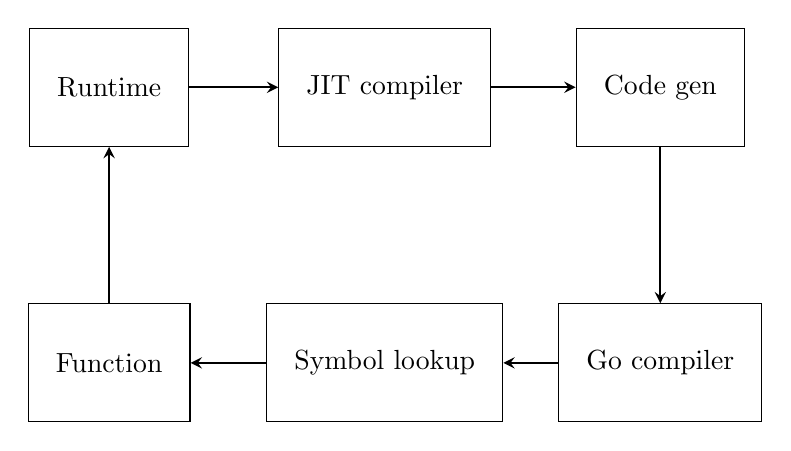
\begin{tikzpicture}[node distance=3.5cm]
        \node (runtime) [process] {Runtime};
        \node (jitcompiler) [process, right of=runtime] {JIT compiler};
        \node (jitcodegen) [process, right of=jitcompiler] {Code gen};
        \node (jitfunction) [process, below of=runtime] {Function};
        \node (symbollookup) [process, right of=jitfunction] {Symbol lookup};
        \node (gocompiler) [process, right of=symbollookup] {Go compiler};

        \draw [arrow] (runtime.east) -- (jitcompiler.west);
        \draw [arrow] (jitcompiler.east) -- (jitcodegen.west);
        \draw [arrow] (jitcodegen.south) -- (gocompiler.north);
        \draw [arrow] (gocompiler.west) -- (symbollookup.east);
        \draw [arrow] (symbollookup.west) -- (jitfunction.east);
        \draw [arrow] (jitfunction.north) -- (runtime.south);
    \end{tikzpicture}
    \caption{Compilation pipeline}
    \label{chart:pipeline-conversion}
\end{figure}

The just in time compiler proceeds to pass the accepted function and the
meta data for its returning types and the passed in arguments to the code
generation step and converts the abstract syntax tree nodes for the function
into their corresponding go representation. After the code generation step
of the compilation pipeline, the go toolchain, including the compiler, is
invoked and thus creates a shared object, generally named a go plugin
\cite{go_plugin}.

Once this plugin is compiled, the symbol lookup stage denotes the process of
loading the plugin and performing a lookup for the compiled function as a
non typed symbol. The last step of this lookup stage is the type conversion
for the return value of the compiled function as well as type casting the
whole function to a function accepting and returing values which types are
erased. After this the function is regarded as compiled and ready to be
attached to the runtime and executed once the runtime invokes the function
again.

\autoref{chart:pipeline-conversion} visualizes the above while highlighting
the dependence of the steps in the JIT compilation pipeline.

% TODO: write more here
